% !TeX root = ../../../book.tex
\subsection{求和杂谈}\label{sec:section1.4.3}

\subsubsection*{奇数求和:观察模式}

既然谈到了整数求和,那就让我们来看一些相关的问题。首先,我们将介绍一种解释奇数之和的有趣得几何方法:让我们将 $1$ 表示为 $1 \times 1$ 块,然后将每个连续增大的奇数表示为角为 $1 \times 1$ 块的直角,完美贴合前一个这样的图。我们为什么要这样做?因为都是奇数,连续项的大小相差为 $2$,每次将角块的边延长 $1$,可以让直角与原图形紧密地相互贴合并逐渐构建起更大的正方形!

\begin{center}
    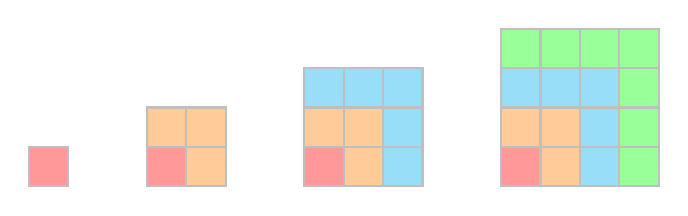
\begin{tikzpicture}[thick,scale=0.5, x=1cm, y=1cm]
        \foreach \x in {0,3,7,12}
        {
            \fill[red!40!white] (\x, 0) rectangle ++ (1,1);
            \draw[lightgray] (\x, 0) rectangle ++ (1,1);
        }

        \foreach \x in {3,7,12}
        {
            \foreach \i in {0,1}
            {
                \fill[orange!40!white] (\x+\i, 1) rectangle ++ (1,1);
                \draw[lightgray] (\x+\i, 1) rectangle ++ (1,1);
                \fill[orange!40!white] (\x+1, \i) rectangle ++ (1,1);
                \draw[lightgray] (\x+1, \i) rectangle ++ (1,1);
            }
        }

        \foreach \x in {7,12}
        {
            \foreach \i in {0,...,2}
            {
                \fill[cyan!40!white] (\x+\i, 2) rectangle ++ (1,1);
                \draw[lightgray] (\x+\i, 2) rectangle ++ (1,1);
                \fill[cyan!40!white] (\x+2, \i) rectangle ++ (1,1);
                \draw[lightgray] (\x+2, \i) rectangle ++ (1,1);
            }
        }

        \foreach \i in {0,...,3}
        {
            \fill[green!40!white] (12+\i, 3) rectangle ++ (1,1);
            \draw[lightgray] (12+\i, 3) rectangle ++ (1,1);
            \fill[green!40!white] (12+3, \i) rectangle ++ (1,1);
            \draw[lightgray] (12+3, \i) rectangle ++ (1,1);
        }
    \end{tikzpicture}
\end{center}

这种模式会持续下去吗?如果我们相信确实如此,我们如何证明这一点呢?这种几何图案的数值之和意味着什么?这是一个首先要回答的好问题,因为尽管几何图案很漂亮,但却很难使用和操作,最终也难以给出明确地\emph{证明}。本质上,对着模式的前几项说:``看,它有效!'' 并不构成官方的数学证明,因此我们必须找到更好的方法来表述这个问题。这并不是要淡化我们注意到的图案的意义和美丽;有趣的是,它的工作方式确实为我们提供了一些有价值的见解,让我们从数学上了解可能发生的事情,但归根结底,这就是它能为我们做的一切。

\subsubsection*{奇数求和:证明我们的发现}

让我们尝试用数字形式写出上图所表示的求和。 角块由 $1 \times 1$ 块组成,每个角比前一个多两块,因此我们看到的每个正方形都可以由一个和表示,例如
\[1 \:\text{ 或 }\: 1+3 \:\text{ 或 }\: 1+3+5 \:\text{ 或 }\: 1+3+5+7 \]
以此类推。我们从这些项中注意到,它们其实是平方数
\[1=1^2 \quad 1+3=4=2^2 \quad 1+3+5=9=3^2 \quad 1+3+5+7=16=4^2 \]
\emph{这}才是我们想要证明的模式;它相当于我们之前注意到的几何图案,但现在它是用我们可以操作的术语编写的。现在让我们思考一下如何才能做到这一点。这种模式与我们之前见过的模式相似吗?我们已经证明了关于整数和的结果了吗?当然!回顾之前的题目;(事实上,在某些方面)我们证明了
\[1 + 2 + 3 + \dots + (n_1) + n =\frac{n^2 + n}{2}\]
这对于该题有何用处?我们证明的求和公式涉及从 $1$ 到 $n$ 的\emph{所有}连续整数,但对于当前要求的公式,我们只想考虑连续\emph{奇数}。

之前我们用函数 $S(n)$ 表示前 $n$ 个自然数之和,所以我们定义函数 $T(n)$ 表示前 $n$ 个奇数之和。现在,我们首先需要确定该和的项,然后以某种方式将它们与 $S(n)$ 联系起来。下面,我们写出了 $n = 1,2,3 ,4$ 时的和。你能找到一种方法来识别求和中的最大项并用 $n$ 表示它吗?
\begin{align*}
    n=1: &\quad 1\\
    n=2: &\quad 1+3\\
    n=3: &\quad 1+3+5\\
    n=4: &\quad 1+3+5+7\\
\end{align*}
请注意,求和项的最后一项始终为 $2n-1$。这与一个普遍事实有关,即对于某个特定整数 $k$,任何偶数整数都可以表示为 $2k$,对于某个特定整数 $n$,任何奇数整数都可以表示为 $2n - 1$。(对于某个整数,我们也可以将奇数表示为 $2n + 1$,不过,这里使用 $2n - 1$ 更方便。)因此,我们要求的前 $n$ 个奇数之和的公式为
\[T(n) = 1 + 3 + 5 + 7 + \dots + (2n - 3) + (2n - 1)\]
我们可以将这个求和公式与 $S(n)$ 或类似的公式联系起来吗?请注意求和公式
\[S(2n) = 1 + 2 + 3 + \dots + (2n - 3) + (2n - 2) + (2n - 1) + 2n\]
包含从 $1$ 到 $2n$ 的\emph{所有}自然数,而 $T(n)$ 仅包含该范围内的奇数。也许两个和相减并尝试找到剩余项之和的表达式是有意义的:
\begin{align*}
    S(2n) - T(n) &= 1 + 2 + 3 + \dots + (2n - 1) + 2n \\
    &\quad -\big(1 + 3 + 5 + \dots + (2n - 3) + (2n - 1)\big) \\
    & =  2 + 4 + 6 + \dots + (2n - 2) + 2n
\end{align*}
这些项都是从 $2$ 到 $2n$ 的\emph{偶数}。我们怎样才能得到这个求和公式呢?我们是否需要做额外的工作,还是可以应用之前的证明结果?由于所有项都是\emph{偶数},我们可以将所有项除以 $2$ 并写成
\begin{align*}
    \frac{1}{2}\big(S(2n) - T(n)\big) &= \frac{1}{2}\big(2 + 4 + 6 + \dots + (2n - 2) + 2n\big)\\
    &= 1 + 2 + 3 + \dots + (n - 1) + n = S(n)
\end{align*}
我们可以保证,最右边的求和公式中的所有项都是整数。不仅如此,它们\emph{都是}从 $1$ 到 $n$ 的连续整数,并且我们知道它们的求和公式!现在,\text{一切都是用我们已知的公式}(即 $S(n)$ 和 $S(2n)$)以及我们要求的公式(即 $T(n)$)书写的。最后一步要做的是整理方程,分离 $T(n)$,然后代入我们已知的 $S$ 的公式:
\begin{align*}
    \frac{1}{2}\big(S(2n) - T(n)\big) &= S(n) \\
    S(2n) - T(n) &= 2S(n) \\
    T(n) &= S(2n) - 2S(n) \\
    T(n) &= \frac{(2n)^2 + 2n}{2} - \frac{2 \cdot (n^2 + n)}{2} \\
    T(n) &= \frac{4n^2 + 2n - 2n^2 - 2n}{2} \\
    T(n) &= \frac{2n^2}{2} \\ 
    T(n) &= n^2
\end{align*}
这看起来相当不错,不是吗?尽管必须完成一些代数步骤,我们还是得出了我们希望证明的结论:连续奇数的和是完全平方数。不仅如此,我们还成功地精确证明了该平方数与求和项数之间的关系。 具体来说,我们刚刚证明的结论的一种简洁概括描述是``前 $n$ 个奇数之和等于 $n^2$''。

\subsubsection*{另一种解法:归纳证明}

我们可以用不同的方式证明这一点吗?如果我们还没有证明上一节的结论,或者我们没有想到以这种方式证明它怎么办?我们能否以某种方式利用我们最初注意到的和的几何结构?

让我们回过头来用稍微不同的方式思考这个问题。具体来说,让我们看看为什么在求和中再添加一项会产生另一个平方数。假设我们已知其中一个求和产生一个平方数;我们知道这对于第一个求和 ($1 = 1^2$) 是正确的,但我们假设对于任意数量的项 $n$ 都会发生这种情况。也就是说,对于某个值 $n$, 我们\emph{假设}
\[1 + 3 + 5 + \dots + (2n - 3) + (2n - 1) = n^2\]
基于这一事实,我们接下来可以推断出下一个和是什么吗?当我们向求和中再添加一项时,我们会加上下一个奇数 $2n + 1$,所以让我们看看这会如何影响求和结果:
\[1 + 3 + 5 + \dots + (2n - 3) + (2n - 1) + (2n + 1) = n^2 + 2n + 1 = (n + 1)^2\]
这似乎证实了我们的想法,不是吗?知道求和的表现方式与我们预期的一致(``如果前 $n$ 个奇数整数之和为 $n^2$……'')我们就可以推断下一个和也必须以相同的方式表出现(……那么前 $n+1$ 个奇数整数的和是 $(n+1)^2$'')。这也证明了结论吗?你觉得怎么样?本质上假设我们的结论成立来进一步证明它,这感觉很奇怪吗?我们真的是这么做的吗?

这种证明策略 --- 使用结果的一种形式来证明结果的``后续''形式 --- 称为\textbf{数学归纳法}。(一般来说,``后续''一词的含义取决于上下文;在这里,它的意思是再加上一项后和。)我们将在下一章更详细地研究这一策略。目前,我们先指出这是一个完美的策略,但它高度依赖于第一个求和的正确表示:$1 = 1^2$。这样,我们所做的工作使我们能够推断出第二个求和是 $(1+3=2^2)$,接着就可以推断出第三个求和是 $(1+3+5=3^2)$,以此类推……如果我们只能证明第二部分,但第一部分的结果没有按照我们想要的方式计算怎么办?我们还能证明结论吗?一般来说,这对归纳策略有何启示?稍后我们将更普遍地解决其中一些问题。

\subsubsection*{泛化:算术级数}

我们要谈的最终求和问题与我们迄今为止看到的两个问题密切相关,事实上,如果我们能证明下一个结论,就不必证明前两个结论了!从这个意义上说,下一个结论比前两个结论更强:这个结论的真实性意味着前两个结论的真实性。(这是数学术语中的常见概念,将结论标记为比其他结论更强或更弱。)

对于这个结论,我们想要发展一个通用\textbf{算术级数}。这句话的意思是我们要添加一个算术级数,其中连续项之间的差是一个固定值。另一种思考方式是,每一项都是通过前一项加上一个固定常数而来。请注意,我们在后两个题目中求和的就是算术级数:第一个求和中,每项相差 $1$(或者,每项上加 $1$ 得到下一项),第二个求和中每个项相差 $2$(或者,每项上加 $2$ 得到下一项)。

我们如何表示一个通用的算术级数?因为连续项必须相差一个固定常数,让我们为该值分配一个变量,例如 $c$,作为常数。求和中也必须有第一项,所以让我们将该值分配给一个变量,例如 $a$,因为它是第一个字母。我们还需另一个变量来告诉我们求和中有多少项,因此我们将使用 $k$ 表示项数,因为我们之前已经使用过该变量表示相同的含义。现在,我们可以用这三个变量来表示整个求和:
\[A(a, c, k) = a + (a + c) + (a + 2c) + (a + 3c) + \dots + (a + (k - 2)c) + (a + (k - 1)c)\]
我们可以利用每对连续项相差 $c$ 这一事实,使用第一项 $a$ 来表示第二项,并且我们可以通过不断增加 $c$ 来表示第三项,依此类推。我们总共需要 $k$ 项,因此,将第一项视为 $a+ 0 \cdot k$,最后一项是我们将 $c$ 添加到第一项 $k - 1$ 次后得到的结果(从 $0$ 到 $k - 1$(含) 有 $k$ 个数字)。另请注意,我们引入了符号 $A(a, c, k)$ 来表示``第一项 $a$、常数差 $c$ 和 $k$ 项的算术级数之和''。现在,我们怎样才能算出这个和呢?

让我们采用以前有效的策略:在第一个求和题目中,我们正序和倒序写下求和项并将它们加在一起。这会创建许多具有相同求和结果的项对,从而将求和简化为乘法。如果我们在这里这样做时会发生什么?我们看到

\begin{center}
    \begin{tabular}{ccccccccc}
                 a & + &      (a+c) & + & \dots & + & (a+(k-1)c) & = & A(a,c,k)\\\noalign{\smallskip\smallskip}
        (a+(k-1)c) & + & (a+(k-2)c) & + & \dots & + &          a & = & A(a,c,k)\\\noalign{\smallskip\smallskip}
        \hline
        (2a+(k-1)c)& + & (2a+(k-1)c)& + & \dots & + &(2a+(k-1)c) & = &2A(a,c,k)\\\noalign{\smallskip\smallskip}
    \end{tabular}
\end{center}
我们再次发现配对项都有相同的和,在这种情况下,和是 $2a+ (k-1)c$。这样的配对项有多少对?正好是 $k$ 个项!(这就是我们选择使用该变量的原因。)将求和表示为乘法,我们现在可以推出
\[2A(a, c, k) = k \cdot (2a + (k - 1)c)\]
因此
\[A(a, c, k) = \frac{k}{2} \cdot k \cdot (2a + (k - 1)c)\]
这看起来符合你的期望结果吗?你的预期是什么?有时,尝试``猜测''可能会发生什么,然后看看结果是否与你的直觉相符,以及如何相符,会有所帮助。

\subsubsection*{具体应用}

上面提到过,我们之前题目中的求和都是算术级数,那么这个公式是否可以得出这些求和的正确结果呢?在第一题中,变量值为 $a = 1,c = 1, k = n$;代入这些值会得到
\[A(1, 1, n) = \frac{1}{2} \cdot k \cdot (2 + (n - 1)) = \frac{n}{2} \cdot(n+1) = \frac{n^2+n}{2}\]
这确实是我们之前得到的结论。那第二题呢?变量的值是多少?公式正确吗?这些问题请你来验证结果。

\subsubsection*{另一种表示}

这个问题的最后,我们想讨论另一种表示刚刚推导出的公式的方法。查看括号中的项,并以稍微不同的方式书写:$a+ (a+ (k-1)c)$。这些项看起来特别有趣吗?是的,它们分别是求和的第一项和最后一项。这为我们提供了一种不同的方式来表达我们推导出的求和公式:$A(a, c, k) = \frac{k}{2}(a + b)$,其中 $a$ 是求和的第一项,$b$ 是最后一项。这个版本的公式可以更方便,更快捷地进行一些求和。

例如,假如我们让你求一个算术级数之和,其中第一项为 $12$,最后一项为 $110$,总共有 $14$ 项,你就不必费心费力去计算常数差 $c$;相反,你可以简单地完成求和:$\frac{14}{2} \cdot (12 + 110) = 854$。是不是快得多?该算术级数的 $c$ 值是多少?给定 $a,b,k$,有没有一种简单的方法可以快速求出 $c$?

\subsubsection*{解题心得}

了解以前的结论会很有帮助,因为它们可以使证明更简短、更容易。有时,很难知道某个特定结果何时有用,或者即使意识到它的用途,也可能很难弄清楚如何应用它。在这种情况下,我们意识到到我们之前已经证明了一个求和公式,因此至少尝试弄清楚它在证明不同的求和公式时如何发挥作用是有意义的。然而,有一种完全不同的方法可以证明奇数之和的公式,不依赖于我们之前的结论。这暗示了一个更通用的结论,好奇的数学家会尝试更通用地探索这个问题,我们通过研究任意算术级数做到了这一点。但最终,我们对前两个求和公式使用了多种策略,并且仅将其中一种策略应用于一般级数问题。我们可以在其他设定下使用这些策略吗?我们是否也可以通过归纳法来证明第一个求和公式?我们可以使用正序/逆序技术来证明第二个求和公式吗?尝试使用这些策略,看看会发生什么。这对你来说可能会很奇怪或没有必要,因为我们已经有了结论,但是了解不同技术在不同环境中如何发挥作用是一个宝贵的经验。在数学中,弄清楚在证明中使用哪种策略通常与找出证明结果一样困难(甚至更难)。考虑到这一点,练习特定的策略来培养一种直觉,知道它们何时有效以及何时需要尝试其他方法,是很有帮助的。
